\section{Proposed fusion framework}
the schematic diagram of the proposed fusion framework is shown in Fig\ref{fig:method} . In the Fig\ref{fig:method} only the fusion of two source images is considered while the proposed framework can be straightforwardly extended to fuse more than two images. The detailed fusion scheme contains the following four steps  \hfill \break


\begin{enumerate}
   \item \textbf{MST decompositon:}   Perform a specific MST on the two source images \( \left\{    {I}_{A},{I}_{B}\right\}  \)to obtain their low-pass bands \(\left\{{L}_{A},{L}_{B}\right\} \) and high-pass bands which are uniformly denoted as
 \(\left\{{H}_{A},{H}_{B}\right \} \)
 \item \textbf{Thresholding:} Perform thresholding as obtain in eq.\ref{bayest} on the low pass and high pass band to remove the unnecessary coefficient from the decomposition.  
    
	\item  \textbf{Low-pass fusion:} 	    
   \begin{itemize}
     \item Apply the sliding window technique to divide \( \left\{ {I}_{A},{I}_{B}\right\}  \)  into image patches of size \(\sqrt{n}\times\sqrt{n}\) from upper left to lower
right with a step length of s pixels. Suppose that there are
T patches denoted as \( \{{P}_{A}^{i}\}_{i=1}^{T}   \)
and  \( \{{P}_{B}^{i}\}_{i=1}^{T} \) in \({L}_{A}\) and \({L}_{B}\) respectively
respectively
     \item For each position i,rearrange \(\{P_{A}^{i},P_{B}^{i} \} \) into column vectors rearrange \(\{ \hat{V}_{A}^{i},\hat{V}_{B}^{i} \} \) by \begin{equation}
     \hat{V}_{A}^{i}=V_{A}^{i}-\bar{V}_{A}^{i}.1
     \end{equation}
     \begin{equation}
     \hat{V}_{B}^{i}=V_{B}^{i}-\bar{V}_{B}^{i}.1
     \end{equation}
     whre 1 denotes an all=one valued \(n \times 1 \) vector \(\bar{V}_{A}^{i}\) and \(\bar{V}_{B}^{i}\) are mean values of all the elements in \({V}_{A}^{i}\) and \({V}_{B}^{i}\) respectively.
     \item Calculate the sparse coefficient vectors \( \{\alpha_{A}^{i},\alpha_{B}^{i} \} \) of \(\{ \hat{V}_{A}^{i},\hat{V}_{B}^{i} \}\)using the orthogonal matching pursuit (OMP) algorithm \cite{24} by
     \begin{equation}
    \alpha _{A}^{i}=\arg \min \parallel \alpha \parallel _{0}   st \parallel \hat{V}_{A}^{i}-D\alpha \parallel_{2} < \epsilon     
\end{equation}      
\begin{equation} \label{eq:6}
\alpha _{B}^{i}=\arg \min \parallel \alpha \parallel _{0}   st \parallel \hat{V}_{B}^{i}-D\alpha \parallel_{2} < \epsilon
\end{equation}
where \textbf{D} is the learned dictionary.
\item Merge \( \alpha_{A}^{i} and \alpha_{B}^{i} \) with the "max-L1" rule to obtain the fused sparse vector
\begin{equation}
\alpha_{F}^{i}=
\begin{cases}
\alpha_{A}^{i} & \text{ if } \parallel \alpha_{A}^{i} \parallel_1 > \parallel \alpha_{B}^{i} \parallel_1\\ 
\alpha_{B}^{i} & \text{ otherwise } 
\end{cases}
\end{equation}
The fused result of \(V_{A}^{i} and V_{B}^{i}\) is calculated by \begin{equation}
V_{F}^{i}=D\alpha_{F}^{i}+\bar{V}_{F}^{i}.1
\end{equation}
where the merged mean value \(\bar{V}_{F}^{i}\) is obtained by 
\begin{equation} \label{eq:8}
\bar{V}_{F}^{i}=
\begin{cases}
\bar{V}_{A}^{i} & \text{ if }  \alpha_{F}^{i} =  \alpha_{B}^{i} \\ 
\bar{V}_{B}^{i} & \text{ otherwise } 
\end{cases}
\end{equation}
\item  Iterate the above process for all the source image patches in \(\{P_{A}^{i} \}_{i=1}^{T} \) and \(\{P_{B}^{i} \}_{i=1}^{T} \)to obtain all the fused vectors \(\{V_{F}^{i} \}_{i=1}^{T} \). Let \(L_{f}\) denotes the low-pass fused result. For each \(V_{F}^{i}\)reshape it into a patch \( p_{F}^{i}\)and then plug  \( p_{F}^{i}\)Finto its original position in \(L_{F}\).As patches are overlapped, each pixel’s value in \(L_{F}\) is averaged over its accumulation times
  \end{itemize}
   
   \item \textbf{High-pass fusion :} Merge \(H_{A} and H_{B}\)to obtain \(H_{F}\) with the popular "max-absolute"
rule using the absolute value of each coefficient as the activity level measurement. Then, apply the consistency verification scheme  to ensure that a fused coefficient does not originate from a different source image from most of its
neighbors. This can be implemented via a small majority filter

\item \textbf{MST reconstruction} Perform the corresponding inverse MST over \(L_{F} and H_{F}\) to reconstruct the final fused image \(I_{F}\)
\end{enumerate}

\begin{figure}[h!]
  \centering
  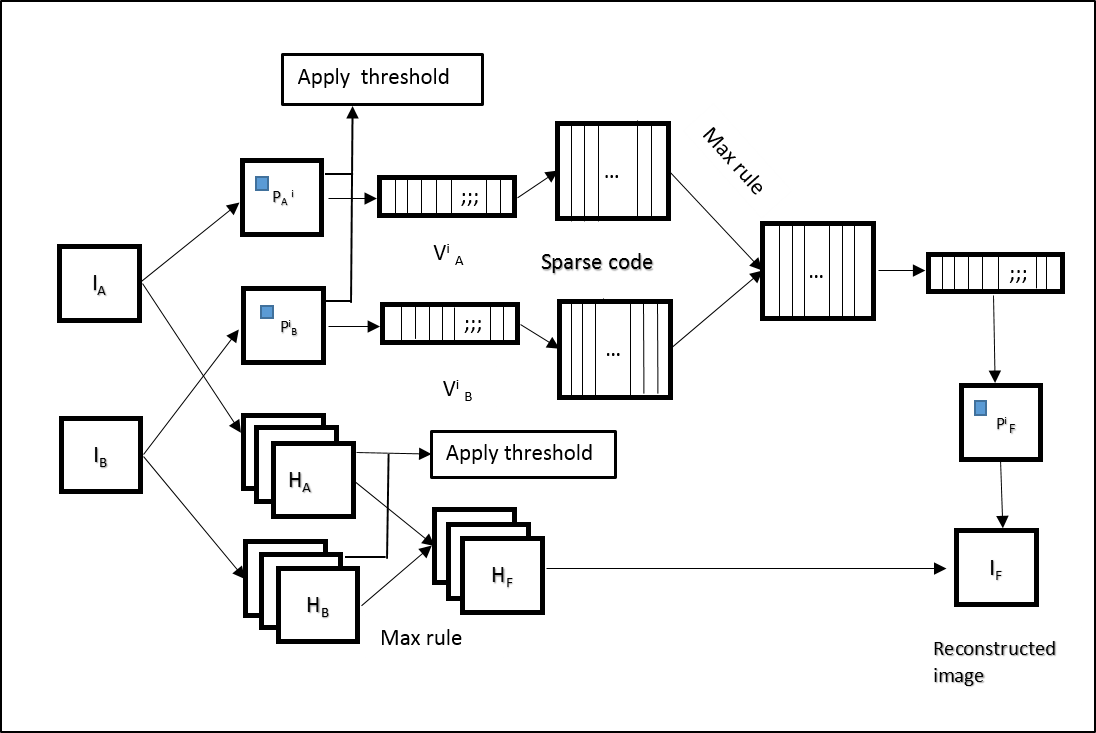
\includegraphics[width=.8\textwidth]{method.png}
  \caption{The schematic diagram of the proposed fusion framework} \label{fig:method}
\end{figure}

\section{Advantage over the MST based methods}
For the conventional MST-based image fusion methods (the
high-pass bands are merged with the "max-absolute" rule while the low-pass bands are fused using the "averaging" rule), there are two main drawbacks as follows \hfill \break

The first one is the loss of contrast. Since most energy of an
image is contained in the low-pass band (even though the decomposition level is set to 4 according to the analysis , the "averaging" fusion rule tends to lose some energy in the source images. For multi-focus image fusion, this phenomenon is not obvious because the source images are captured from the same type of sensors. However, for the fusion of multimodal images such as visible-infrared and medical images, the fused results of the MST-based methods are often in low contrast. This is mainly because different imaging modalities reflect different physical attributes, so a same region in different source images may have different brightness. For example,Fig. \ref{fig:advntg} shows a pair of computed tomography (CT) and magnetic resonance (MR) images. It can be seen that the CT image mainly focuses on dense structures like bones, while the MR image provides excellent soft-tissue details. When the "averaging" rule is used for low-pass fusion, the energy contained in those regions will be lost to a large extent.
As a result, the contrast of those regions in the fused image will decrease a lot after MST reconstruction \hfill \break

The second one is the difficulty in selecting the MST decomposition level. On one hand, to ensure enough spatial details can be extracted from the source images, the decomposition level cannot be too small such as 1 or 2. On the other hand, Li et al.\cite{25} experimentally verified that when the decomposition level is too large, one coefficient in the low-pass band have an impact on a large set of pixels in the fused image, so an error in the low-pass band (mainly caused by noise or mis-registration between the source images) will lead to serious artificial effects. Moreover, when the decomposition level becomes larger, the quality of high-pass fusion is also more sensitive to noise and mis-registration. Therefore, when the source images are not precisely registered, the decomposition level cannot be too large. Particularly, for multi-focus image fusion, due to the different imaging parameters (e.g. focal length) for multiple source images, the locations of object edges in different
source images are often not exactly the same for their different sharpness. A typical example is shown in Fig.\ref{advntg} Between the two source images, both the borders and numbers of the two clocks in the scene have different sharpness, so it is practically impossible to make an accurate registration. Thus, a compromise on decomposition level should be made for the consideration of extracting enough spatial details and being robust to mis-registration.\hfill \break

As a smart blending approach, the SR-based image fusion
scheme is combined into the MST-based fusion methods to
overcome the above two defects. In the proposed framework, the
SR-based scheme is employed to fuse the MST low-pass bands.In
Section2, after applying the "max-L1" rule in Eq.\ref{eq:6}, we transfer the energy in source images to the fused image by Eq.\ref{eq:8}.Therefore, the contrast in the fused image is improved. For the second defect, by extracting spatial details in low-pass band with the SR-based fusion scheme, the decomposition level can be set less than 4 for multi-focus image fusion to make the method more robust to mis-registration. Thus, the difficulty in determining decomposition level can be well solved.

\section{Advantages over the SR-based method}
The conventional SR-based image fusion method[14] mainly
has the following three defects.\hfill \break

The first one is the fine details in source images like textures and edges tend to be smoothed for the following two reasons. First, the signal representation ability of the dictionary may be not sufficient for fine details, which means that the reconstruction result is not approximate to the input signal. As we know, the representation ability of the over-completed dictionary relies much on the number of atoms in it, but a dictionary with a large size will directly increase the computational cost. More importantly, the study in[22]shows that a highly redundant dictionary may lead to potential visual artifacts in the reconstruction result, especially
when the input signal is corrupted by noise. Thus, a compromise on dictionary size is usually required. A typical example is that the dictionary size is 256 when the input signal is 64 dimensional \(8 \times 8\). Second, the usage of sliding window technique may also cause smoothness. The step length of the sliding window is usually set to 1 when fusing images directly in spatial domain to avoid blocking effects. However, when the adjacent patches are greatly overlapped, some details in the fused image will be smoothed. \hfill \break

The second one is the "max-L1" rule may cause spatial inconsistency in the fused image when the source images are captured by different imaging modalities. As mentioned before, for multimodal image fusion, a region may be very bright in one source image while very dark in another, but the region in both of them may be very "flat" with few fine details. Note that although a region in each of two source images is visually "flat", there still exists little difference between the two source images in terms of variance, and the difference is usually consistent over all the patches in that region. That is to say, if one patch in the region of source image A
has a larger variance than the corresponding patch in source image B, then most of the other patches in that region of source image A also tend to have larger variances than the corresponding patches in source image B. However, since the difference is very tiny, the "max-L1" fusion rule will become very sensitive to the random noise in spatial domain because a small change of value at a pixel may influence the fusion result of several patches. As a result, the fused patches in that region may originate from different source images, which will lead to spatial inconsistency in the fused image. Since the SR-based method handles patches in spatial domain, the
impact of high-frequency noise is considerable. \hfill \break

The third one is the low computational efficiency. Since the sliding window’s step length should be small enough, the sparse coding technique is performed on a large number of image patches. For instance, when the patch size is \(8\times8 \) and the step length is set to 1, there are 62001 patches to be processed for a source image of size \(256 \times256\) . In this case, it usually takes several minutes to fuse two source images with the SR-based method \hfill \break

The proposed fusion framework can effectively overcome the
above three defects of the SR-based method. In our fusion framework, the high-frequency spatial information is separated by performing MST and extracted by the "max-absolute" rule.
Meanwhile, the representation ability of the dictionary is enough to satisfy the reconstruction accuracy for low-frequency components. Furthermore, we will show in the next section that the sliding window’s step length in low-pass bands can be set larger than that in spatial domain. Therefore, the inclination of SR-based method to smooth fine details can be prevented. For the second defect, without high-frequency details, the random noise can be effectively eliminated, so the probability that the patches in a "flat" 
region originate from different source images will decrease to a large extent, leading to better spatial consistency. Finally, the computational efficiency can also be improved by the proposed framework because the number of patches required to be processed with the sparse coding technique is greatly reduced. For one thing, the step length can be set larger. For another, the low-pass bands of many MSTs such as LP and DWT have smaller size relative to the original image. \\ \\ 

\begin{figure}[ht] 
  \begin{subfigure}[b]{0.25\linewidth}
    \centering
    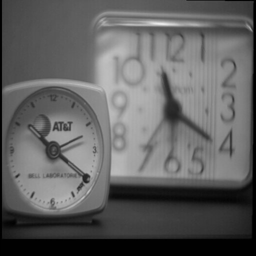
\includegraphics[width=0.5\linewidth]{5a.png}
    \caption{} 
    \label{1a} 
    \vspace{4ex}
  \end{subfigure}%%
  \begin{subfigure}[b]{0.25\linewidth}
    \centering
    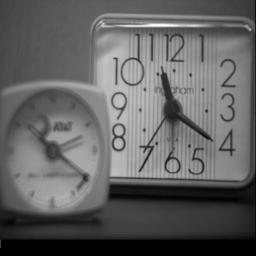
\includegraphics[width=0.5\linewidth]{5b.png}
    \caption{} 
    \label{1b} 
    \vspace{4ex}
  \end{subfigure}%%
  \begin{subfigure}[b]{0.25\linewidth}
    \centering
    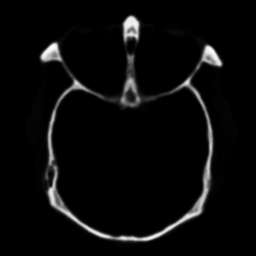
\includegraphics[width=0.5\linewidth]{5c.png} 
    \caption{} 
    \label{1c} 
    \vspace{4ex}
  \end{subfigure}%%
  \begin{subfigure}[b]{0.25\linewidth}
    \centering
    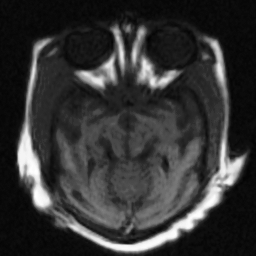
\includegraphics[width=0.5\linewidth]{5d.png}
    \caption{} 
    \label{1d} 
    \vspace{4ex}
  \end{subfigure}%%
  \caption{Two pairs of source images. (a,b)multi-focus images , and (c,d)  Medical images .}
  \label{advntg} 
\end{figure}

